%! Author = nadutkinfedor
%! Date = 28.02.2024

% Preamble
\documentclass[11pt]{article}
\usepackage[left=2cm, right=1cm, top=2cm, bottom=2cm, bindingoffset=0cm]{geometry}

% Packages
\usepackage[utf8]{inputenc}
\usepackage[russian]{babel}
\usepackage{amsmath}
\usepackage{hyperref}
\usepackage{graphicx}
\usepackage{misccorr}
\usepackage{listings}
\usepackage{xcolor}
\usepackage{titlesec}
\usepackage{minted}
\usepackage{color}
\usepackage{enumitem}
\usepackage{indentfirst}

%listing settings
\definecolor{dkgreen}{rgb}{0,0.6,0}
\definecolor{gray}{rgb}{0.5,0.5,0.5}
\definecolor{mauve}{rgb}{0.58,0,0.82}

\lstset{language=SQL,
    basicstyle={\small\ttfamily},
    belowskip=3mm,
    breakatwhitespace=true,
    breaklines=true,
    classoffset=0,
    columns=flexible,
    commentstyle=\color{dkgreen},
    framexleftmargin=0.25em,
    keywordstyle=\color{blue},
    numbers=none, %If you want line numbers, set `numbers=left`
    numberstyle=\tiny\color{gray},
    showstringspaces=false,
    stringstyle=\color{mauve},
    tabsize=3,
    xleftmargin =1em,
    backgroundcolor=\color{gray!10}
}

\lstset{ %
    backgroundcolor=\color{white},   % choose the background color
    basicstyle=\footnotesize,        % size of fonts used for the code
    breaklines=true,                 % automatic line breaking only at whitespace
    captionpos=b,                    % sets the caption-position to bottom
    commentstyle=\color{dkgreen},    % comment style
    escapeinside={\%*}{*},          % if you want to add LaTeX within your code
    keywordstyle=\color{blue},       % keyword style
    stringstyle=\color{mauve},     % string literal style
}

% link setting
\hypersetup{
    colorlinks=true,
    linkcolor=blue,    % Синий цвет для внутренних ссылок
    filecolor=magenta, % Можно выбрать другой цвет для файлов
    urlcolor=blue      % Синий цвет для URL
}

% Title
\title{DB internals. Пятая
лекция}
\author{Надуткин Федор }
\date{February 2024}

\titleformat{\section}[block]{\Huge\bfseries\filcenter}{}{1em}{}
\titleformat{\subsection}[block]{\LARGE\bfseries\filcenter}{}{1em}{}
\titleformat{\subsubsection}[block]{\Large\bfseries\filcenter}{}{1em}{}

% Document
\begin{document}

    \maketitle
    \newpage


    \section{Pull based execution}

    Представляем каждый оператор в виде итератора по строчкам.
    Оператор подтягивает изменения от детей.
    Каждый раз когда нам нужны данные от детей, мы вызываем \texttt{nextRow} на детях.

    \begin{lstlisting}[language=Java]
        interface Operator {
            Optional<Row> nextRow();
        }
    \end{lstlisting}

    Внутренняя структура каждого оператора

    \begin{lstlisting}[language=Java]
        class SomeOperator implements Operator {
            private Operator child;

            @Override
            Optional<Row> nextRow() {
                var row = child.nextRow();
                // Do operator logic
                return result;
            }
        }
    \end{lstlisting}

    \begin{figure}[h!]
        \centering
        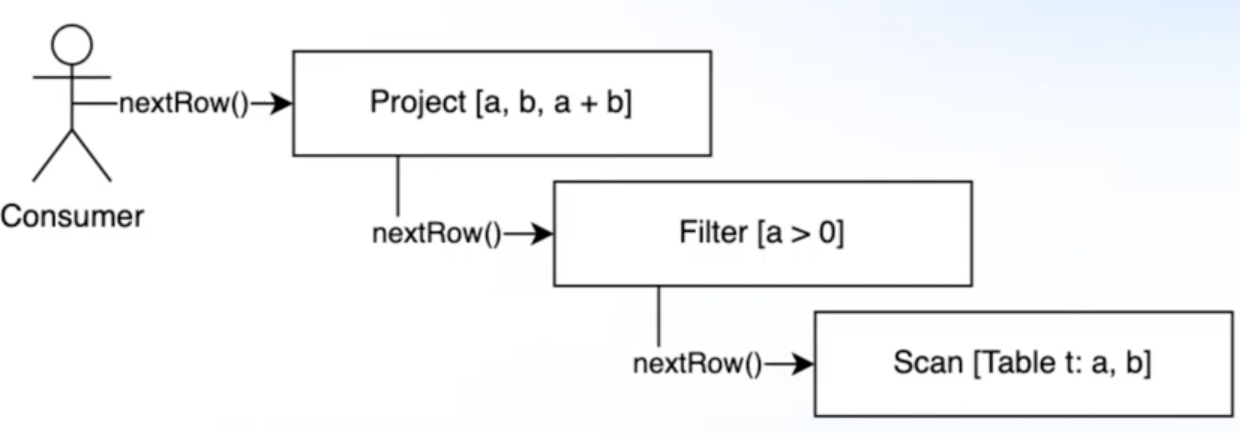
\includegraphics[width=\textwidth]{Pictures/Pull/Consumer pulls}
        \caption{Пример работы и подтягивании изменений}
    \end{figure}

    \begin{itemize}[label=+]
        \item Простота реализации
    \end{itemize}
    \begin{itemize}[label=-]
        \item Высокие накладные расходы на вызов \texttt{nextRow()}.
        Решение - возвращать список строк.
        \item Непредсказуемое исполнение.
        Не каждый вызов \texttt{nextRow} может вообще что-то вернуть (например \texttt{Filter}).
        \item Приостановка исполнения становится головной болью.
        \item Непонятно как распараллеливать выполнение оператора, что достаточно критично при обработке большого количества строк одним оператором.
    \end{itemize}

    \newpage

    \section*{Push based execution}

    Оператор не знает, кто его \texttt{input}, он только принимает на исполнение и в ответ отдаёт \texttt{output}

    \begin{lstlisting}[language=Java]
        interface Operator {
            void addInput(List<Row> rows);
            boolean needsInput();
            Optional<List<Row>> getOutput();
            Future<Void> isBlocked();
            boolean isFinished();
        }
    \end{lstlisting}

    \begin{itemize}
        \item \texttt{boolean needsInput()} --- некоторые операторы могут производить более, чем 1 выход в обмен на input, этот флаг позволит понять нужно ли оператору ещё данных или он всё ещё производит.
        \item \texttt{boolean isFinished()} --- приостановление оператора.
        \item \texttt{boolean isBlocked()} --- работа с сетью/диском/параллельно.
    \end{itemize}

    Такая модель позволяет нам делать параллельное исполнение, главное не нарушать инварианты, которые были бы при последовательном исполнении.

    \begin{figure}[h!]
        \centering
        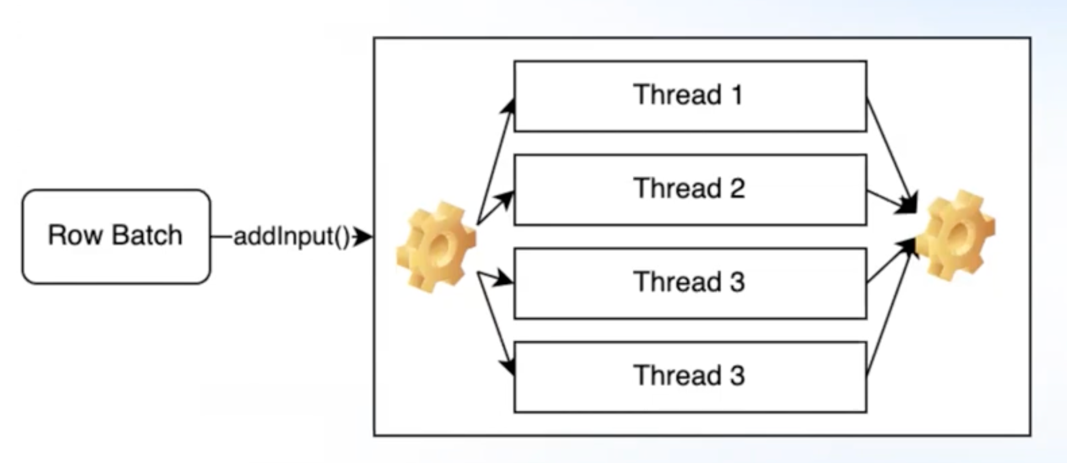
\includegraphics[width=0.8\textwidth]{Pictures/Push/Push parallelism}
        \caption{Распараллеливание работы при push execution.}
    \end{figure}

    Некоторые операторы могут выдавать \texttt{output} сразу как был дан \texttt{input}.
    Например \texttt{Scan} или \texttt{Filter}.
    Другие же операторы могут корректно отработать только тогда, когда им дадут полностью весь \texttt{input}, например \texttt{Aggregate}.
    Отсюда можно делить операторы на \textbf{streaming} и \textbf{blocking}.

    \newpage

    \subsection{Блокирующие операторы}

    \begin{figure}[h!]
        \centering
        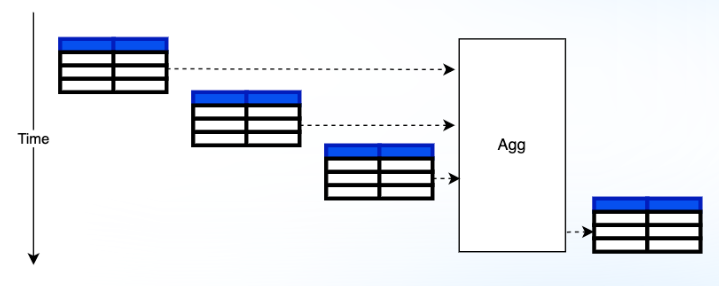
\includegraphics[width=0.8\textwidth]{Pictures/Push/Operators/Blocking operators}
        \caption{Пример работы блокирующего оператора}
    \end{figure}

    \begin{itemize}
        \item \texttt{HashAggregate}
        \item \texttt{Window}
        \item \texttt{Sort}
    \end{itemize}

    \subsection{Потоковые операторы}

    \begin{figure}[h!]
        \centering
        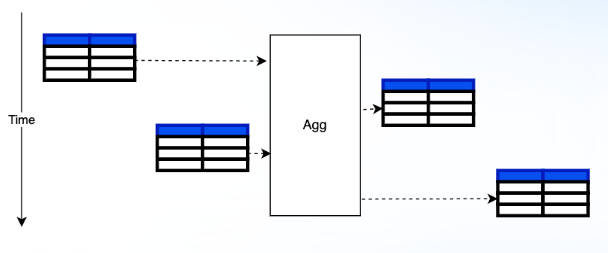
\includegraphics[width=0.8\textwidth]{Pictures/Push/Operators/Streaming operator}
        \caption{Пример работы потокового оператора}
    \end{figure}

    \begin{itemize}
        \item \texttt{Scan}
        \item \texttt{Filter}
        \item \texttt{Union All}
        \item \dots
    \end{itemize}

    \subsection{HashJoin}

    Отдельная история с \texttt{HashJoin}, ведь после того, как хеш таблица для одного ребёнка построена, можно делать исполнение параллельным.
    Появляется идея разбиения исполнения на 2 части блокирующую и потоковую.

    \begin{figure}[h!]
        \centering
        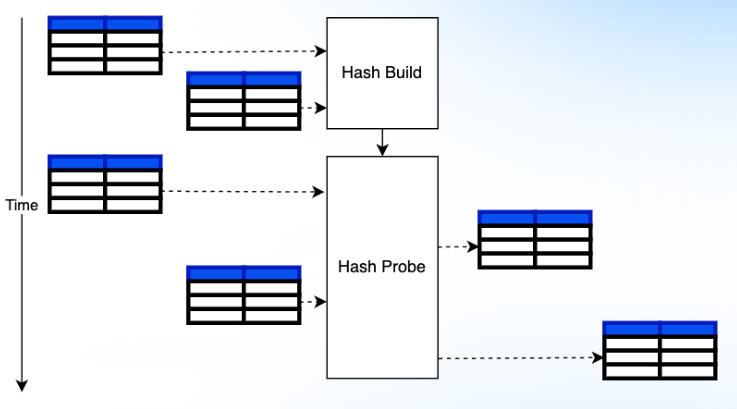
\includegraphics[width=0.6\textwidth]{Pictures/Push/Operators/HashJoin}
        \caption{Разбиваем HashJoin на 2 части: построение таблицу и сам Join}
    \end{figure}

    \subsection{Pipelining}

    Логично разбить последовательности на куски (pipeline), заканчивающиеся блокирующими операторами.
    Между ними могут существовать зависимости, а значит, что порядок на них важен.

    \begin{figure}[h!]
        \centering
        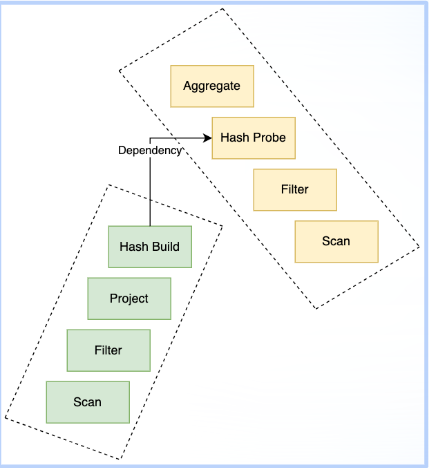
\includegraphics[width=0.4\textwidth]{Pictures/Push/Operators/Pipelining}
        \caption{Пример разбиения работы на pipe}
    \end{figure}

    \newpage


    \section{Parallelism}

    Разделяют 2 способа распараллеливания исполнения.

    \begin{figure}[h!]
        \begin{minipage}{0.5\textwidth}
            \centering
            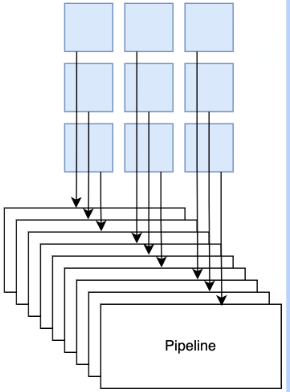
\includegraphics[width=0.6\textwidth]{Pictures/Push/Parallelism/Data Parallelism}
            \caption{Параллелизм данных - расскидывание данных на разные pipeline}
        \end{minipage}
        \begin{minipage}{0.5\textwidth}
            \centering
            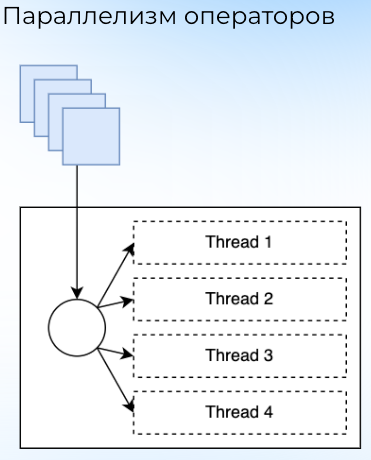
\includegraphics[width=0.6\textwidth]{Pictures/Push/Parallelism/Operator Parallelism}
            \caption{Параллелизм операторов - Закидывание данных на один оператор, а тот в свою очередь расскидывает по потокам}
        \end{minipage}
    \end{figure}

    \subsection{Параллелизм операторов}

    \textbf{Что нужно:}
    \begin{itemize}
        \item Чтобы у каждого оператора был доступ к пулу потоков.
        \item Чтобы создание потока было гораздо дешевле, чем синхронная обработка потока (иначе параллелизм не имеет смысла).
    \end{itemize}

    \subsubsection{Сортировка}

    \begin{figure}[h!]
        \centering
        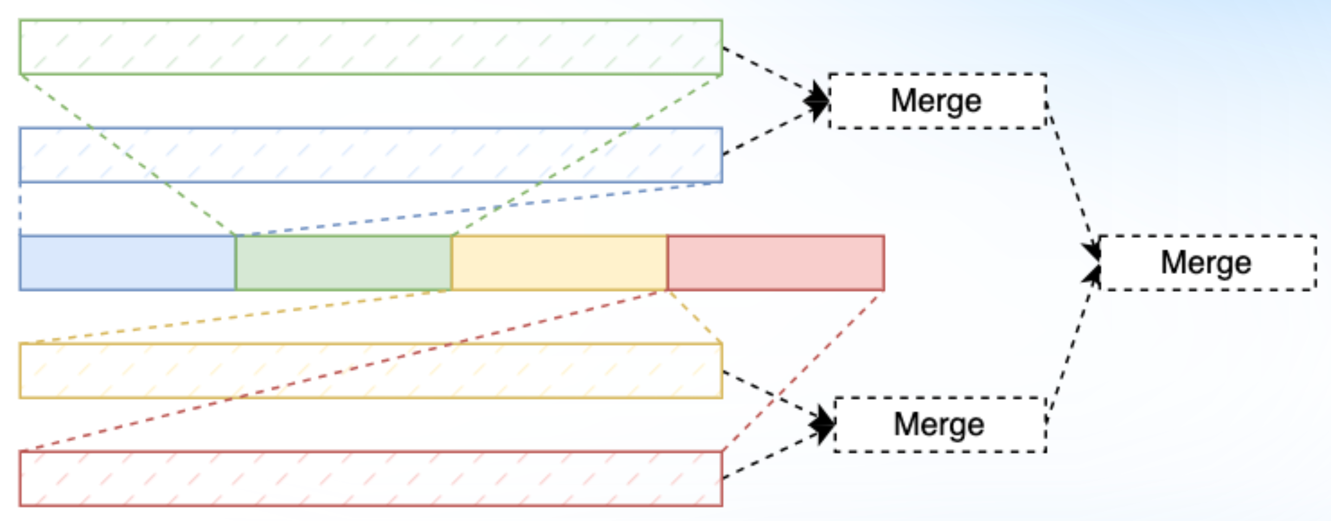
\includegraphics[width=0.7\textwidth]{Pictures/Push/Parallelism/Operators/Сортировка}
        \caption{Пример распараллеливания сортировки}
    \end{figure}
    
    \subsubsection{Хеш-аггрегат}
    
    \begin{figure}[h!]
        \centering
        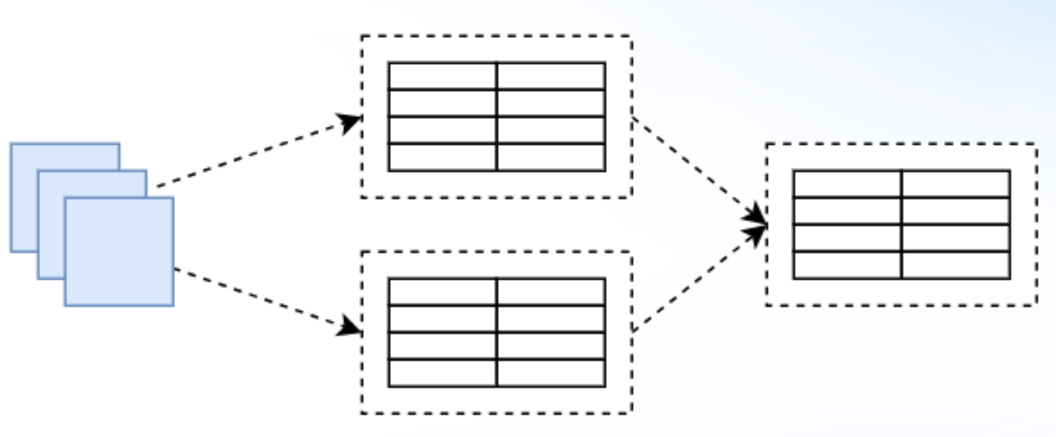
\includegraphics[width=0.7\textwidth]{Pictures/Push/Parallelism/Operators/Хеш аггрегат}
        \caption{Пример распараллеливания хеш аггрегата. В конце таблицы надо смёржить}
    \end{figure}

    \subsection{Параллелизм данных}

    Каждый поток читает независимый кусок данных и выполняет его в своём pipeline.
    Такой подход может быть не всегда корректен, так как могут возникать конфликты, пример на картинке.
    
    \begin{figure}[h!]
        \centering
        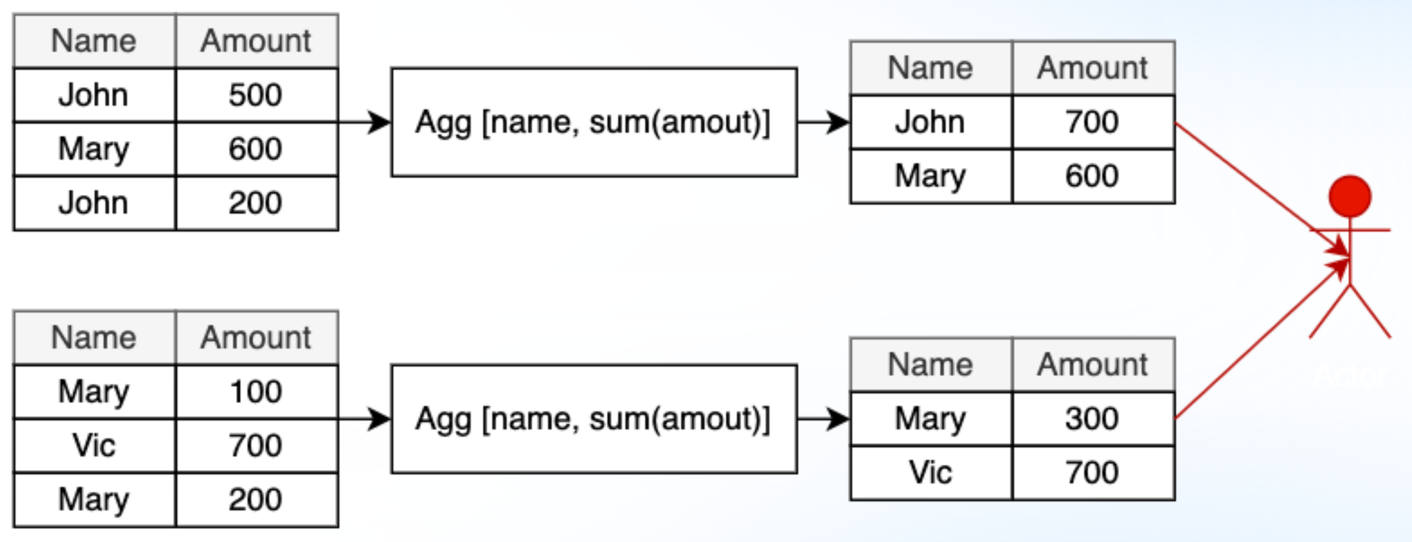
\includegraphics[width=0.7\textwidth]{Pictures/Push/Parallelism/Data/Conflict}
        \caption{Конфликтная ситуация при параллелизме данных}
    \end{figure}

    В таком случае там нужно делать точки остановки в которых эти конфликты будут решаться.

    Отдельной историей для рассмотрения параллелизма данных может быть распределённая система, когда данные разделены на разные шарды (или реплики).
    Для подобных случаев стоит разбивать на куски, какие-то из них будут выполняться на одном шарде, а после этого будет сделан \texttt{Exchange}, который выстроит логику работу правильно.
    
    \begin{figure}[h!]
        \centering
        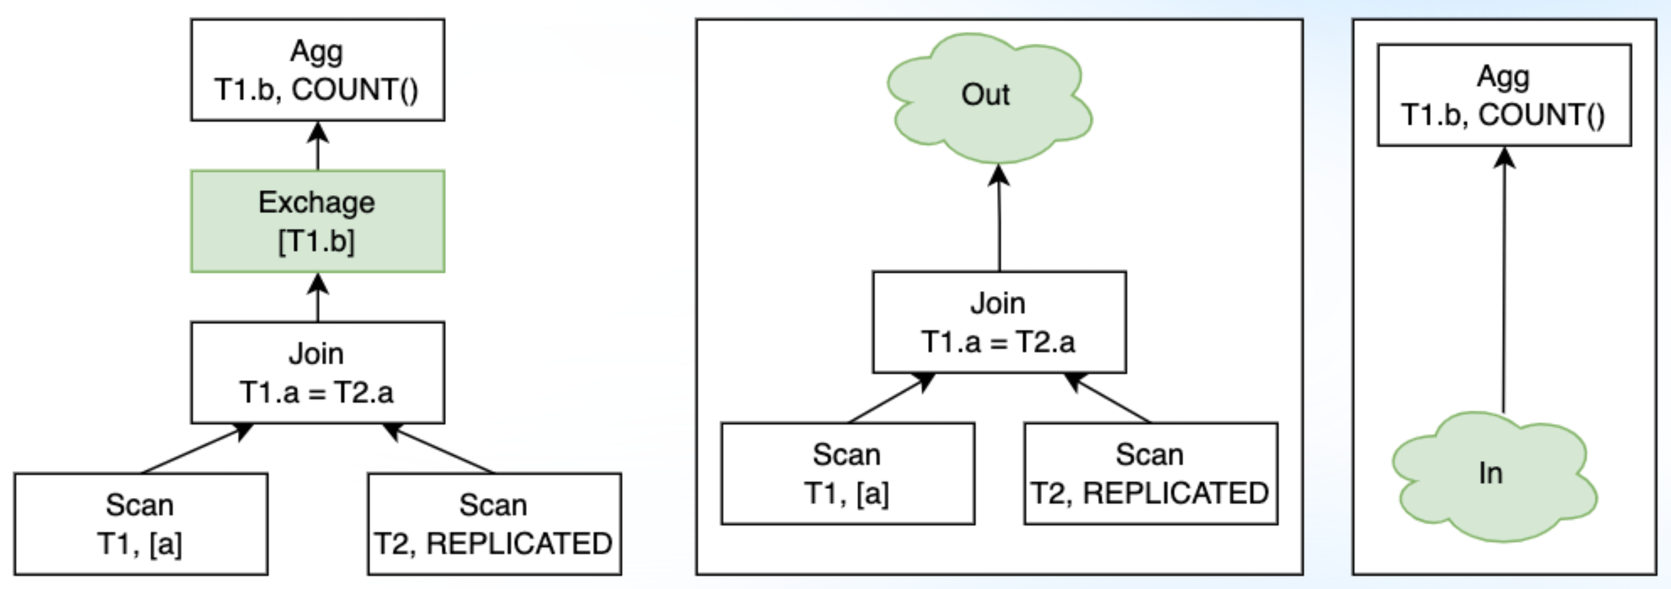
\includegraphics[width=0.5\textwidth]{Pictures/Push/Parallelism/Data/Exchange}
        \caption{Пример Exchange оператора}
    \end{figure}
    


\end{document}